% !TeX spellcheck = en_GB
\section{indexing \& searching}

In this section we will discuss how Hibernate Search's engine (in the form of the module "hibernate-search-engine") can be used in general. Then we will work out a standalone version of this engine that is easier to work with and lastly we will show how we integrate this standalone version with JPA.

\subsection{Setting up the example project}

Before we start describing how we do things in particular, we set up the example entities described in \ref{example_project} as if the original Hibernate Search would have been used. We do so by adding additional annotations to our entity-classes:

\begin{enumerate}
	\item \textbf{@Indexed}: marks the entity as an index root-type.
	\item \textbf{@DocumentId}: marks the field as the id of this entity. this is only needed if no JPA @Id can be found, but can be used to override settings.
	\item \textbf{@Field}: describes how the annotated field should be indexed. if no "name" is specified, the fieldname defaults to the property name.
	\item \textbf{@IndexedEmbedded}: marks relational properties that should be included in the index. if no name is specified, all fields contained in these entities are prefixed with the property this is placed on.
	\item \textbf{@ContainedIn}: used in entities that are embedded in other indexes. this is set on the properties that point back to the index-owning entity.
\end{enumerate}
\noindent
The resulting entities look like this:
\\
\lstset{language=java}
\lstset{moredelim=[is][\bfseries]{[*}{*]}}
\begin{lstlisting}[frame=htrbl, caption={Book.java with Hibernate Search annotations}, label={lst:book.java_2}]
@Entity
@Table(name = "Book")
[*@Indexed*]
public class Book {

	@Id
	@Column(name = "isbn")
	[*@DocumentId*]
	private String isbn;
	
	@Column(name = "title")
	[*@Field(store = Store.YES, index = Index.YES)*]
	private String title;
	
	@Column(name = "genre")
	[*@Field(store = Store.YES, index = Index.YES)*]
	private String genre;
	
	@Lob
	@Column(name = "summary")
	[*@Field(store = Store.NO, index = Index.YES)*]
	private String summary;
	
	@ManyToMany(mappedBy = "books", cascade = {
		CascadeType.MERGE,
		CascadeType.DETACH,
		CascadeType.PERSIST,
		CascadeType.REFRESH
	})
	[*@IndexedEmbedded(includeEmbeddedObjectId = true)*]
	private Set<Author> authors;
	
	//getters & setters ...
}
\end{lstlisting}

\lstset{language=java}
\lstset{moredelim=[is][\bfseries]{[*}{*]}}
\begin{lstlisting}[frame=htrbl, caption={Author.java with Hibernate Search annotations}, label={lst:author.java_2}]
@Entity
@Table(name = "Author")
public class Author {

	@Id
	@GeneratedValue(strategy = GenerationType.AUTO)
	@Column(name = "authorId")
	[*@DocumentId*]
	private Long authorId;
	
	@Column(name = "firstName")
	[*@Field(store = Store.YES, index = Index.YES)*]
	private String firstName;
	
	@Column(name = "lastName")
	[*@Field(store = Store.YES, index = Index.YES)*]
	private String lastName;
	
	@Column(name = "country")
	[*@Field(store = Store.YES, index = Index.YES)*]
	private String country;
	
	@ManyToMany(cascade = {
		CascadeType.MERGE, 
		CascadeType.DETACH, 
		CascadeType.PERSIST, 
		CascadeType.REFRESH
	})
	@JoinTable(name = "Author_Book", 
		joinColumns = 
			@JoinColumn(name = "authorFk", 
				referencedColumnName = "authorId"),
		inverseJoinColumns = 
			@JoinColumn(name = "bookFk", 
				referencedColumnName = "isbn"))
	[*@ContainedIn*]
	private Set<Book> books;
	
	//getters & setters ...
}
\end{lstlisting}
\noindent
As these annotations are defined in hibernate-search-engine, we can rely on all of them in while designing the standalone integration of Hibernate Search.

\subsection{Using Hibernate Search's engine}

As already described earlier (\ref{problem_indexing_searching}), hibernate-search-engine is not intended to be used by application developers, but for other APIs to integrate with. Therefore there is no real public documentation available on how to use it and all following information had to be retrieved from tests in the hibernate-search-engine and hibernate-search-orm integration module source code.

\subsubsection{Starting the engine}
A Hibernate Search engine instance is represented by a \textbf{SearchIntegrator}. In order to obtain it, we first have to create special configuration class that implements the \textbf{org.hibernate.search.cfg.spi.SearchConfiguration}. An object of this class has then to be created and filled with all the configuration properties Hibernate Search requires. The minimum that has to be set in this class's property map are the following two settings:

\begin{enumerate}
	\item \textbf{hibernate.search.default.directory\_provider}: The two most common cases here are either "ram" or "filesystem". This decides where the index will be stored. A ram directory is only present in the system memory while the SearchIntegrator exists while the "filesystem" option is persistent. For "filesystem" the additional property "hibernate.search.default.indexBase" has to be set to an appropriate path.
	
	\item \textbf{hibernate.search.lucene\_version}: This decides which Lucene version should be used internally. The currently latest supported version is "4.10.4".
\end{enumerate}
\noindent
A complete list of the available settings can be found in the Hibernate Search documentation\footnote{Hibernate Search documentation, see~\cite{hibernate_search_doc}} (only some Hibernate ORM specific settings cannot be used). Our \textbf{StandaloneSearchConfiguration} (\ref{lst:StandaloneSearchConfiguration.java}) defaults to "ram" and "4.10.4".
\\\\
After such a class is created, a \textbf{SearchIntegrator} can be obtained by a \textbf{SearchIntegratorBuilder} like this:
\\
\lstset{language=java}
\lstset{moredelim=[is][\bfseries]{[*}{*]}}
\begin{lstlisting}[frame=htrbl, caption={Starting up the engine}, label={lst:starting_up_engine.java}]
List<Class<?>> indexClasses = Arrays.asList(Book.class, Author.class);

SearchConfiguration searchConfiguration = 
		new StandaloneSearchConfiguration();
indexClasses.forEach( searchConfiguration::addClass );

//bootstrapping class for Hibernate Search
SearchIntegratorBuilder builder = new SearchIntegratorBuilder();

//we have to build an integrator here (the builder needs a 
//"base integrator" first before we can add index classes)
builder.configuration( searchConfiguration ).buildSearchIntegrator();

indexClasses.forEach( builder::addClass );

//starts the engine with all configuration properties set
SearchIntegrator searchIntegrator = builder.buildSearchIntegrator();

//use the integrator ...

//close it
searchIntegrator.close();
\end{lstlisting}

\subsubsection{Indexing, updating and deleting objects from the index}

Now that we know how a SearchIntegrator can be built, we can take a look at how we can control the index using the engine's features. The engine does a lot of optimizations in the backend. This is the reason it abstracts the index control methods away in a \textbf{Worker} pattern that accepts \textbf{Work} objects (the different actions are represented by different \textbf{WorkType}s). Such a worker can batch operations by synchronizing upon the  \textbf{org.hibernate.search.backend.TransactionContext} interface. Our implementation of that is simply called \textbf{Transaction} (\ref{lst:Transaction.java}).
\\\\
We index objects with \textbf{WorkType.INDEX}:
\\
\lstset{language=java}
\begin{lstlisting}[frame=htrbl, caption={Indexing an object with the engine}, label={lst:indexing_object_native.java}]
Book book = ...;
Transaction tx = new Transaction();
Worker worker = searchIntegrator.getWorker();
worker.performWork( new Work( book, WorkType.INDEX ), tx );
tx.commit();
\end{lstlisting}
~\\
We update objects with \textbf{WorkType.UPDATE}:
\\
\lstset{language=java}
\begin{lstlisting}[frame=htrbl, caption={Updating an object with the engine}, label={lst:updating_object_native.java}]
Book book = ...;
Transaction tx = new Transaction();
Worker worker = searchIntegrator.getWorker();
worker.performWork( new Work( book, WorkType.UPDATE ), tx );
tx.commit();
\end{lstlisting}
~\\
We delete objects with \textbf{WorkType.PURGE}:
\\
\lstset{language=java}
\begin{lstlisting}[frame=htrbl, caption={Deleting an object by id with the engine}, label={lst:deleting_object_native.java}]
String isbn = ...;
Transaction tx = new Transaction();
Worker worker = searchIntegrator.getWorker();
worker.performWork( new Work( Book.class, isbn, WorkType.PURGE ), tx );
tx.commit();
\end{lstlisting}

\subsubsection{Querying the index}

\lstset{language=java}
\begin{lstlisting}[frame=htrbl, caption={Querying the index with the engine}, label={lst:querying_natively.java}]
SearchIntegrator searchIntegrator = ...;

//find information about all the entities matching a given title
List<EntityInfo> entityInfos = 
	searchIntegrator.createHSQuery().luceneQuery( 
			searchIntegrator.buildQueryBuilder()
				.forEntity( Book.class )
				.get()
				.keyword()
				.onField( "title" )
				.matching( "searchString" )
				.createQuery()
		).targetedEntities(
			Collections.singletonList(
				Book.class
			)
		).projection(
			ProjectionConstants.ID
		).queryEntityInfos();

//extract info from the entityInfos
for(EntityInfo entityInfo : entityInfos) {
	String isbn = (String) entityInfo.getProjection()[0];
	//handle this information ...
}
\end{lstlisting}

\subsection{Standalone version of Hibernate Search}


\textcolor{red}{Architektur, Klassendiagramm, zusätzliche Features (DtoDescriptor)}

\begin{figure}[ht]
	\centering
	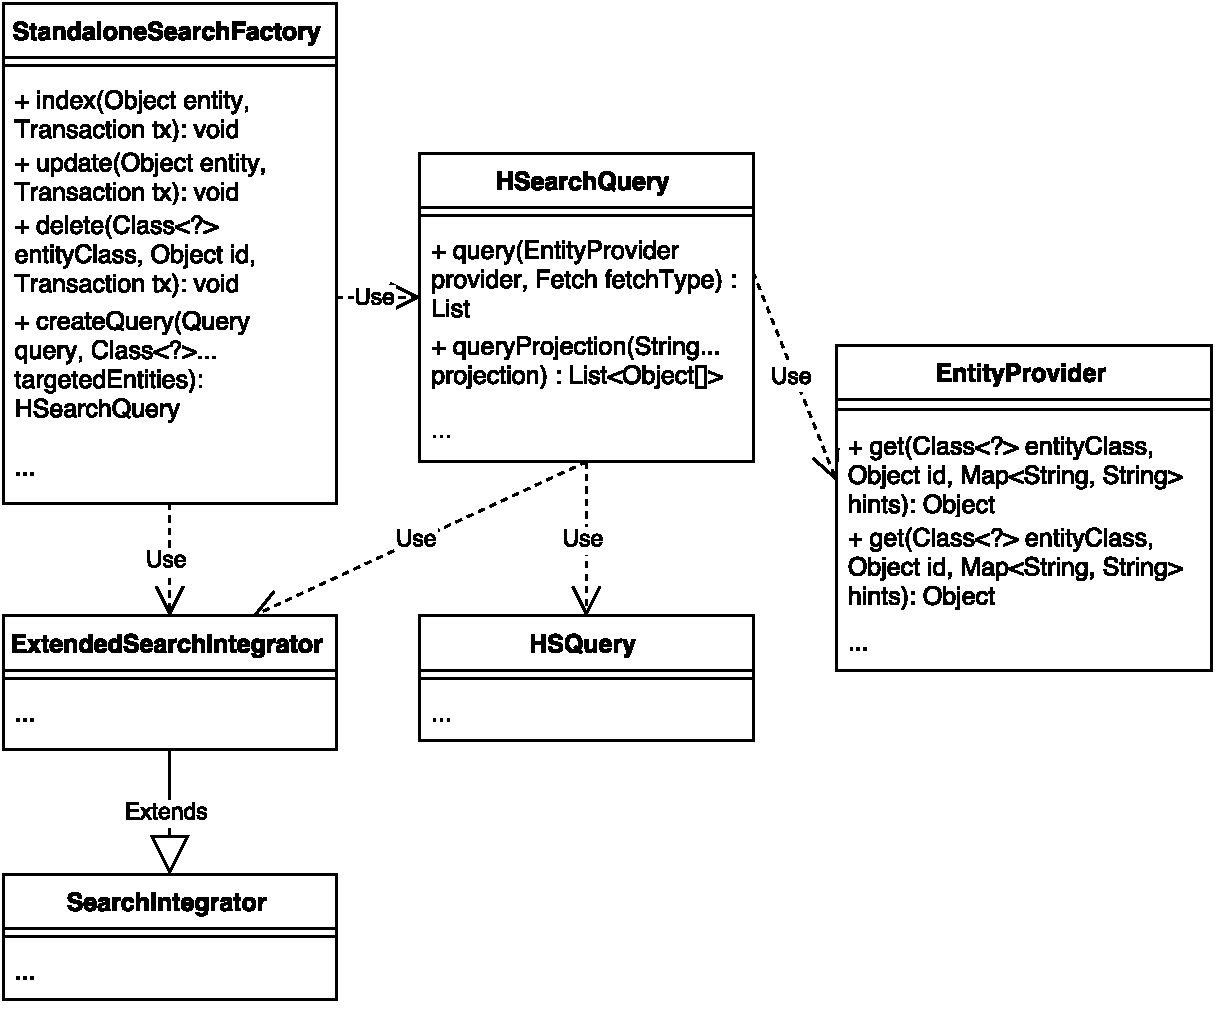
\includegraphics[scale=0.7]{images/standalone_min_architecture.pdf}
	\caption{Rough architecture of the standalone}
	\label{standalone_min_architecture}
\end{figure}

\subsubsection{Starting the standalone}

\lstset{language=java}
\lstset{moredelim=[is][\bfseries]{[*}{*]}}
\begin{lstlisting}[frame=htrbl, caption={Starting up the standalone}, label={lst:using_standalone.java}]
List<Class<?>> indexClasses = Arrays.asList(Book.class, Author.class);

SearchConfiguration searchConfiguration = 
		new StandaloneSearchConfiguration();
indexClasses.forEach( searchConfiguration::addClass );

StandaloneSearchFactory searchFactory = 
		StandaloneSearchFactoryFactory.
				createSearchFactory(
					searchConfiguration,
					indexClasses
				);
				
//use the searchfactory ...

//close it
searchFactory.close();
\end{lstlisting}

\subsubsection{Indexing, updating and deleting objects from the index}

\lstset{language=java}
\begin{lstlisting}[frame=htrbl, caption={Indexing an object with the standalone}, label={lst:indexing_object_native.java}]
Book book = ...;
searchFactory.index(book);
\end{lstlisting}

\lstset{language=java}
\begin{lstlisting}[frame=htrbl, caption={Updating an object with the standalone}, label={lst:updating_object_native.java}]
Book book = ...;
searchFactory.update(book);
\end{lstlisting}

\lstset{language=java}
\begin{lstlisting}[frame=htrbl, caption={Deleting an object by id with the standalone}, label={lst:deleting_object_native.java}]
String isbn = ...;
searchFactory.delete(Book.class, isbn);
\end{lstlisting}

\subsubsection{Querying the index}

\lstset{language=java}
\begin{lstlisting}[frame=htrbl, caption={Querying the index with the standalone}, label={lst:querying_natively.java}]
StandaloneSearchFactory searchFactory = ...;
EntityProvider entityProvider = ...;

List<Book> = searchFactory.createQuery(searchFactory.buildQueryBuilder()
				.forEntity(Book.class)
				.get()
				.keyword()
				.onField("title")
				.matching("searchString")
				.createQuery(), Book.class
			).query(
				entityProvider,
				Fetch.BATCH
			);
\end{lstlisting}

\subsection{Standalone integration with JPA interfaces}

\textcolor{red}{zusätzliche annotations, restriktionen!}

\pagebreak